\section{Report layout}

After providing a brief introduction to Stratoshperic Airships outlining the aims and objectives of this study, Chapter 2 ?????
 Chapter 3 gives the detailed literature survey of various fields required for multi-disciplinary shape optimization. Chapter 4  explains two of the many methods used for the parameterization of geometry. This is also shown in Figure \ref{Report layout}. Next, crisp introduction for advantages of using OpenFOAM\textsuperscript{\textregistered} is discussed in chapter 5. 

Mesh generation using two utilities namely Gmsh and \textit{SnappyHexMesh} are discussed in chapter 6. Collectively Chapters 3, 4 describe the work dork done in Stage-01. A brief introduction of methodology for optimization is given in chapter 07. However optimization will be done in stage -02 along with other considerations as shown in \ref{Report layout}. 

Finally chapter 8 discusses the results obtained while validating the results present in literature for various standard airship shapes using OpenFOAM\textsuperscript{\textregistered}. Finally chapter 8 gives the future work that will be performed in stage -02. The workflow for the total project is shown in Figure \ref{Report layout}. The blocks present in transparent oval is the work completed in stage 1. 

\begin{figure}[htbp]
	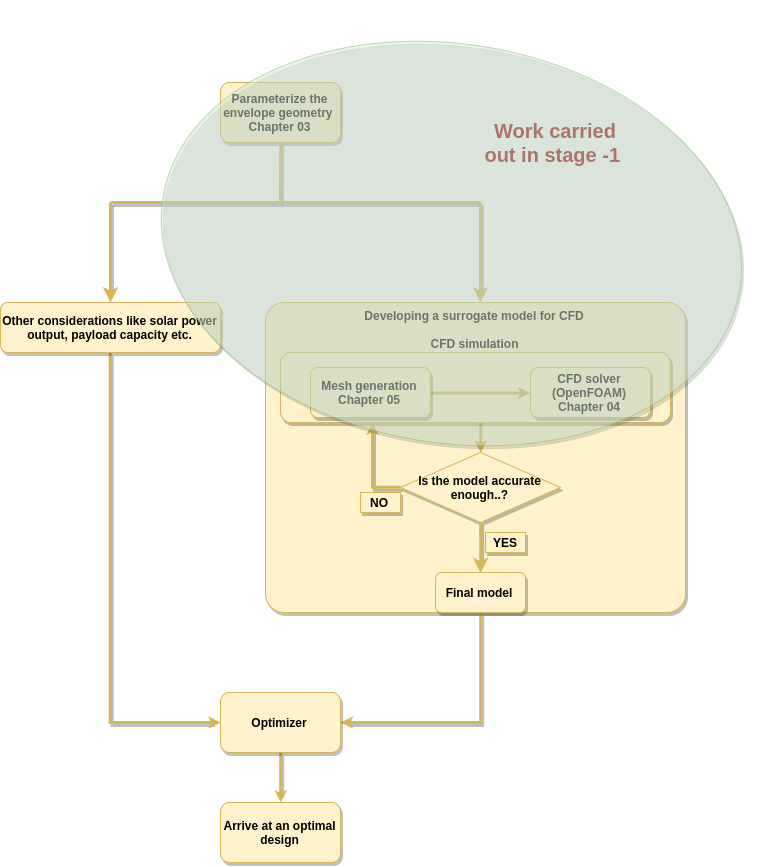
\includegraphics[width=\textwidth]{layout/layout.png} 
	\caption{Work flow of multi-disciplinary shape optimization}
	\label{Report layout} %      only if needed 	
\end{figure}
%%


%%% Local Variables: 
%%% mode: latex
%%% TeX-master: "../mainrep"
%%% End: 
